\documentclass[a4paper,11pt]{article}
\usepackage[french,english]{babel} 
\usepackage{microtype}

\usepackage[utf8]{inputenc}
\usepackage{array}
\usepackage{amsmath} 
\usepackage{amssymb}
\usepackage{amsfonts}
\usepackage{amsthm}
\usepackage{fullpage}%
\usepackage[T1]{fontenc}%

\usepackage{graphicx}%
\usepackage{url}%
\usepackage{abstract}%

\usepackage{mathpazo}%
\parskip=0.5\baselineskip


\title{Binary Decision Diagrams}
\author{Rémi Hutin \& Joshua Peignier}
\date{6 Mai 2016}


\begin{document}
\maketitle

	\section{Introduction}
	Ce document traite la version informatique du sujet proposé, et présente donc des réponses détaillées aux question 1 à 3, ainsi que les points intéressants et résultats de la partie qui concerne le code.\newline
	Pour compiler et exécuter notre code, extrayez le contenu de l'archive fournie dans un répertoire de votre choix. Rendez-vous dans ce répertoire à l'aide d'un terminal, puis compilez avec \texttt{make}, et exécutez avec \texttt{./main}. Notre code, en plus des fonctions demandées dans le sujet, présente un exemple de la résolution du problèmes des $n$ dames pour $n = 12$.\newline
	\emph{Remarque préliminaire} : Dans tout ce document, on admettra l'existence d'une bijection entre l'ensemble des formules INF et l'ensemble des BDD.
	 
	\section{BDD et forme normale if-then-else}

		\paragraph{Question 1}

		Soient $\varphi$ une formule et $x$ une variable.\newline
Nous voulons montrer que $\varphi \equiv\varphi\uparrow^{x}$.\newline
		Remarquons que, par définition, $\varphi\uparrow^{x} \equiv (x \wedge \varphi[1/x]) \vee (\neg x \wedge \varphi[0/x])$.
		
		Voici donc la table de vérité de $\varphi\uparrow^{x}$ en fonction des valeurs de $x$ et de $\varphi$ pour chaque valuation (on ne remplit que les cases nécessaires).\newline
		
		\begin{tabular}{|c|c|c|c|c|c|c|}
		\hline
		$x$ & $\varphi$ & $\varphi[1/x]$ &  $x \wedge \varphi[1/x]$ & $\varphi[0/x]$ & $\neg x \wedge \varphi[0/x]$ & $\varphi\uparrow^{x}$ \\
		\hline
		0 & 0 &   & 0 & 0 & 0 & 0 \\
		\hline
		0 & 1 &   & 0 & 1 & 1 & 1 \\
		\hline
		1 & 0 & 0 & 0 &   & 0 & 0 \\
		\hline
		1 & 1 & 1 & 1 &   & 0 & 1 \\
		\hline
		\end{tabular}
		
		Il suffit alors de remarquer que les colonnes de $\varphi$ et $\varphi\uparrow^{x}$ sont égales.
		
		\paragraph{Question 2}
		
		Nous voulons montrer que toute formule est équivalente à une formule INF.
		Procédons par induction.
		(Suivant la remarque préliminaire établie en introduction, on confondra les formules INF et leurs BDD associés.)
		
		\emph{Remarque} :  Dans cette démonstration, lorsque nous traiterons le cas des connecteurs binaires, nous seront amenés à remplacer des feuilles d'une formule INF ${f'}_1$ par une deuxième formule INF ${f'}_2$ (le tout pour former une formule INF $\varphi'$).
		Notons que nous devons toutefois procéder à des simplifications : si ${f'}_2$ contient une formule INF $F = x \rightarrow F_1,F_0$, et que $x$ est également présente dans ${f'}_1$, alors dans le diagramme de $\varphi'$, nous devons nous assurer de ne pas tester $x$ deux fois sur le même chemin. Donc dans une branche qui se trouve sur le fils faible de $x$ dans ${f'}_1$, si un noeud $x$ réapparaît plus loin, nous supprimons ce deuxième noeud $x$ ainsi que son fils fort $F_1$, et nous le remplaçons par son fils faible $F_0$ (et symétriquement si nous sommes sur une branche sur le fils fort de $x$ dans ${f'}_1$). Nous sous-entendrons ces suppressions de noeuds par la suite, mais elles sont nécessaires pour la construction de la formule INF.
		
		\begin{itemize}
		\item Si notre formule $\varphi$ est réduite à une variable $x$, sans utilisation d'opérateurs, alors $\varphi$ est équivalente à la formule INF $x \rightarrow 1,0$.
		\item Si la formule $\varphi$ s'écrit $\neg f$ et que nous supposons que $f$ est équivalente à une formule INF $f'$, alors $\varphi$ est équivalente à la formule INF $\varphi'$ obtenue en transformant, dans le BDD correspondant à $f'$, les feuilles $0$ en $1$ et les feuilles $1$ en $0$. Ainsi, $\varphi$ est vraie si et seulement si $f$ est fausse, si et seulement si $f'$ est fausse, si et seulement si $\varphi'$ est vraie. 
		\item Si $\varphi$ s'écrit $f_1 \wedge f_2$ et que nous supposons que $f_1$ et $f_2$ sont toutes les deux équivalentes à des formules INF ${f'}_1$ et ${f'}_2$, alors nous pouvons construire une formule INF $\varphi'$ équivalente à $\varphi$ à partir de ${f'}_1$ ; il suffit, dans le BDD correspondant à ${f'}_1$, de remplacer les feuilles $1$ par le BDD complet de ${f'}_2$.
		
		Ainsi, si on parcourt $\varphi'$ avec une valuation telle que ${f'}_1$ soit fausse, on tombe sur $0$, donc $\varphi'$ est fausse. Et si on la parcourt avec une valuation qui rende ${f'}_1$ vraie, alors on arrive sur la racine de ${f'}_2$, et on continue les tests, donc $\varphi'$ a la même valeur que ${f'}_2$. Donc $\varphi'$ est vraie si et seulement si ${f'}_1$ et ${f'}_2$ sont vraies. Donc $\varphi'$ est bien équivalente à $\varphi$.
		\item Si $\varphi$ s'écrit $f_1 \vee f_2$ et que nous supposons que $f_1$ et $f_2$ sont toutes les deux équivalentes à des formules INF ${f'}_1$ et ${f'}_2$, nous procédons de la même manière qu'avant en construisant une formule $\varphi'$ à partir de ${f'}_1$, mais cette fois, il faut remplacer ses feuilles $0$ par la formule INF de ${f'}_2$.
		
		Ainsi, si on choisit une valuation qui rende ${f'}_1$ est vraie, le parcours dans $\varphi'$ avec cette valuation nous amène à un noeud 1, donc est $\varphi'$ est vraie. Sinon, on arrive sur la racine de ${f'}_2$ et on teste cette dernière ; alors $\varphi'$ a la valeur de ${f'}_2$. Donc $\varphi'$ est vraie si et seulement si au moins l'une des deux formules entre ${f'}_1$ et ${f'}_2$ est vraie.
		Donc $\varphi'$ est équivalente à $\varphi$.
		\item Si $\varphi$ s'écrit $f_1 \Rightarrow f_2$ et que nous supposons que $f_1$ et $f_2$ sont toutes les deux équivalentes à des formules INF ${f'}_1$ et ${f'}_2$, nous procèdons de la même manière qu'avant en construisant une formule $\varphi'$ à partir de ${f'}_1$ ; mais cette fois, il faut changer les feuilles $0$ de ${f'}_1$ en $1$, et remplacer ses feuilles $1$ par ${f'}_2$.
		
		Ainsi, une valuation qui rend ${f'}_1$ fausse nous amène sur la valeur $1$ dans $\varphi'$, donc $\varphi'$ est vraie. Et une valuation qui rend ${f'}_1$ vraie nous amène à tester la valeur de ${f'}_2$, qui est celle que prendra $\varphi'$. Donc $\varphi'$ est fausse si et seulement si ${f'}_1$ est vraie et ${f'}_2$ fausse. D'où l'équivalence de $\varphi'$ et $\varphi$.
		\item Si $\varphi$ s'écrit $f_1 \Leftrightarrow f_2$ et que nous supposons que $f_1$ et $f_2$ sont toutes les deux équivalentes à des formules INF ${f'}_1$ et ${f'}_2$, nous procèdons de la même manière qu'avant en construisant une formule $\varphi'$ à partir de ${f'}_1$ : il faut remplacer les feuilles $1$ de ${f'}_1$ par la formule ${f'}_2$, et remplacer les feuilles $0$ de ${f'}_1$ par la formule ${f'}_2$ en prenant soin d'échanger les valeurs $1$ et $0$ sur les feuilles de cette dernière.
		On peut ainsi vérifier que $\varphi'$ est équivalente à $\varphi$.
 		\end{itemize}

Nous pouvons donc en conclure que toute formule est équivalente à une formule INF.
	
		\paragraph{Question 3} Nous allons procéder par récurrence sur $n$.
		Soit donc la propriété $P(n)$ : "pour un ordre sur les variables $x_1 < ... < x_n$ donné, pour toute fonction booléenne $f : \mathbb{B}^n \rightarrow \mathbb{B}$, il existe un unique ROBDD $u$ tel que $f^u = f$."
		
		\begin{itemize}
		\item Montrons $P(1)$ : \newline
		Si $f$ ne prend qu'une variable $x$, alors remarquons qu'il y aura au plus un test. En effet, il est interdit de tester une même variable plusieurs fois sur un même chemin.
		\begin{itemize}
		\item Si $f$ est constante, le BDD réduit au noeud étiqueté par la constante $f$ convient. Il est trivialement ordonné, et trivialement réduit (il n'y a qu'un seul noeud, donc le principe d'unicité est respecté, et ce noeud est une constante, donc il respecte nécessairement le principe d'utilité). C'est donc un ROBDD. Tout autre BDD qu'on pourrait construire imposerait exactement un test sur $x$ (nous n'avons pas le droit d'en faire plus), mais ce test est inutile car la valeur de $f$ est constante. Ce BDD ne serait donc pas réduit. Donc on a l'existence et l'unicité d'un ROBDD $f$ tel que $f^u = f$.
		\item Si $f$ prend deux valeurs différentes, il est nécessaire de faire un test sur sa seule variable, $x$. Un BDD qui convient a donc forcément $x$ pour racine. De plus, comme dit précédemment, il est interdit de faire plus d'un test. Les deux seuls BDD que nous pouvons alors construire avec $x$ pour racine et sans autre test sont ceux associés aux formules INF $x \rightarrow 1,0$ et $x \rightarrow 0,1$. Ils sont tous les deux ordonnés et réduits. Mais un seul des deux BDD correspond à $f$. On a donc l'existence et l'unicité d'un ROBDD $f$ tel que $f^u = f$.
		\end{itemize}
		\item Supposons $P(n)$ pour $n$ donné, et montrons $P(n+1)$ :
		Soient $n+1$ variables $x_1$ à $x_{n+1}$ et l'ordre $x_1 < ... < x_{n+1}$.
		Soit $f$ une fonction booléenne à $n+1$ variables, notées $b_1$ à $b_{n+1}$. Nous considèrons les fonctions booléennes à $n$ variables $f_0$ et $f_1$ telles que $f_0(b_2,...,b_{n+1}) = f(0,b_2,...,b_{n+1})$ et $f_1(b_2,...,b_{n+1}) = f(1,b_2,...,b_{n+1})$.\newline
		
		$f_0$ et $f_1$ sont des fonctions booléennes à $n$ variables, et  les variables $x_2$ à $x_{n+1}$ suivent l'ordre $x_2 < ... <  x_{n+1}$. Donc d'après $P(n)$, il existe un unique ROBDD $u_0$ tel que $f^{u_0} = f_0$, et de même il existe un unique ROBDD $u_1$ tel que $f^{u_1} = f$.\newline

		Nous pouvons donc construire un BDD pour $f$ en prenant $x_1$ pour racine, et en lui donnant pour fils faible la racine de $u_0$ et pour fils fort la racine de $u_1$. On peut vérifier avec les définitions de $f_0$ et $f_1$ que le BDD $u$ ainsi construit est tel que $f^u = f$. De plus, l'ordre donné sur les variables $x_1$ à $x_{n+1}$ est respecté dans $u$, car il a pour racine $x_1$ et que chacun de ses fils est ordonné suivant $x_2 < ... < x_{n+1}$. Nous obtenons alors un $OBDD$, qu'on peut réduire en fusionnant tous les noeuds qui auraient la même étiquette, le même fils fort et le même fils faible, et en supprimant tous les test inutiles (ceux-ci sont déjà a priori supprimés dans les ROBDD $u_0$ et $u_1$ ; il faudrait donc seulement supprimer la racine $x_1$ si son test est inutile). Nous avons donc construit un ROBDD. 

L'unicité de celui-ci est imposée par l'ordre qu'on s'est donné. Si le test de $x_1$ est inutile, on est ramené au cas de $P(n)$, qui est notre hypothèse, et qui assure l'existence et l'unicité du ROBDD construit. Sinon, un tel $ROBDD$ doit forcément avoir $x_1$ pour racine ; et comme fils fort et fils faible, il doit avoir deux autres ROBDD associés respectivement à $f_1$ et $f_0$. Mais ceux-ci sont uniques, d'après la propriété $P(n)$. Il ne peut donc pas en exister d'autre non plus pour $f$. On a donc démontré $P(n+1)$.
		\end{itemize}
		
Nous pouvons en conclure que pour tout $n$, pour un ordre sur les variables $x_1 < ... < x_n$ donné, pour toute fonction booléenne $f : \mathbb{B}^n \rightarrow \mathbb{B}$, il existe un unique ROBDD $u$ tel que $f^u = f$.
		
	\section{Implémentation de ROBDD}
	
	Nous avons réussi à implémenter l'ensemble des fonctions demandées, en particulier l'extension des $n$ dames ; les résultats que nous obtenons semblent cohérents.
	
	Pour le problème des $n$ dames, nous avons créé la fonction \texttt{dames : int -> prop formula}, qui génère la formule modélisant le problème pour une taille donnée. L'idée intuitive pour modéliser le problème est qu'il doit y avoir exactement $1$ dame présente dans chaque ligne et chaque colonne de l'échiquier, et qu'il doit y avoir au plus $1$ dame présente dans chaque diagonale. 
	
	Notre fonction traduit donc cette idée en formule logique. On commence donc par associer à chaque case une variable logique. Par exemple, nous $n = 4$ :
	
	\begin{center}
	\begin{tabular}{|*{4}{c|}}
	
            \hline
            $x_0$ & $x_1$ & $x_2$ & $x_3$ \\
            \hline
            $x_4$ & $x_5$ & $x_6$ & $x_7$ \\
            \hline
            $x_8$ & $x_9$ & $x_{10}$ & $x_{11}$ \\
            \hline
            $x_{12}$ & $x_{13}$ & $x_{14}$ & $x_{15}$ \\
            \hline
        \end{tabular}
        \end{center}
        
        Puis, notre fonction va générer les formules correspondantes. Par exemple, pour la première ligne, la formule générée est :
        
        $$(x_0 \land \neg x_1 \land \neg x_2 \land \neg x_3) \lor (\neg x_0 \land x_1 \land \neg x_2 \land \neg x_3) \lor (\neg x_0 \land \neg x_1 \land x_2 \land \neg x_3) \lor (\neg x_0 \land \neg x_1 \land \neg x_2 \land x_3)$$
        
        On réitère ce procédé pour toutes les lignes, colonnes et diagonales, et on construit une formule globale obtenue par la conjonction de toutes les formules ainsi obtenues. Cette formule est ensuite traduite en ROBDD par la fonction \texttt{build}, et une solution est trouvée par la fonction \texttt{anysat}.
	
	Dans un premier temps, nous avons implémenté les fonctions sans utiliser la programmation dynamique. Les résultats étaients corrects, mais les performances
	étaient assez faibles (nous n'avons pu résoudre le problème des $n$ dames que pour $n \leq 6$).
        Ensuite, nous avons utilisé la programmation dynamique avec des tables de hachages, dans le but d'éviter de faire plusieurs fois les mêmes calculs. Nous avons pu observer une très nette amélioration des performances, et avons pu résoudre le problème pour $n = 12$ en un temps correct, comme le montre la Figure 1.
        
        
        \begin{figure}[t!]
        \centering
        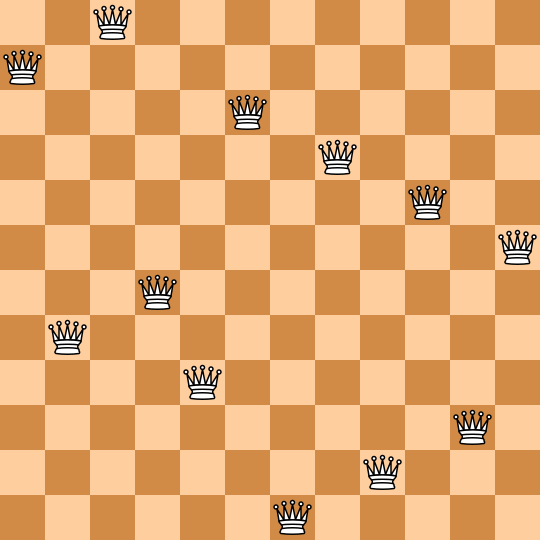
\includegraphics[scale=0.3]{board.png}
        \caption{Une solution au problème des $12$ dames}
        \end{figure}
	
	
\end{document}
